\documentclass[11pt]{article}

\usepackage{amsmath}
\usepackage{textcomp}
\usepackage{tikz}
\usepackage[top=0.8in, bottom=0.8in, left=0.8in, right=0.8in]{geometry}
% add other packages here

% put your group number and names in the author field
\title{\bf Exercise 2: A Reactive Agent for the Pickup and Delivery Problem}
\author{Group \textnumero: Ogier Bouvier, Val\'erian Rousset}

% the report should not be longer than 3 pages

\begin{document}
\maketitle

\section{Problem Representation}

\subsection{Representation Description}
% describe how you design the state representation, the possible actions, the reward table and the probability transition table

For the state representation, we took it from what seems closest to reality

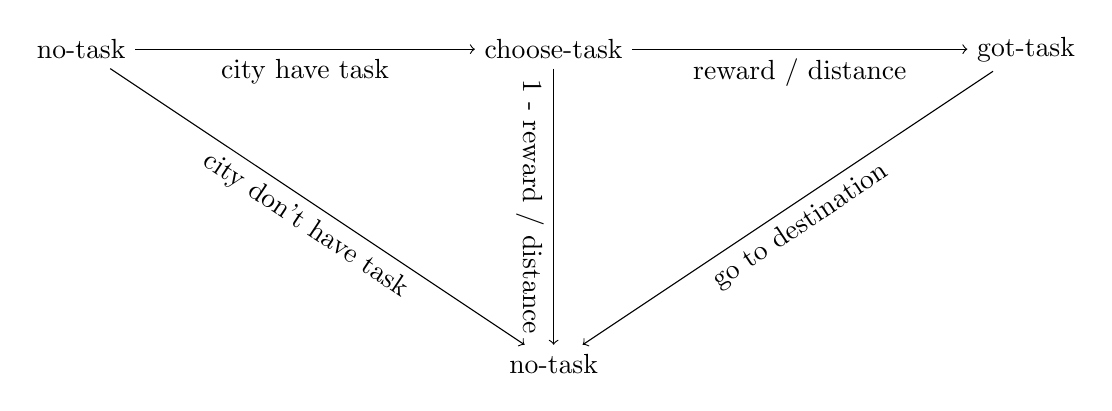
\begin{tikzpicture}
	\node (no-task) at (0,0) {no-task};
	\node (choose-task) at (6,0)  {choose-task};
	\node (got-task) at (12,0)  {got-task};
	\node (no-task-end) at (6,-4) {no-task};

	\draw[->] (no-task) -- (choose-task) node[midway,sloped,below]{city have task};
	\draw[->] (no-task) -- (no-task-end) node[midway,sloped,below]{city don't have task};
	\draw[->] (choose-task) -- (got-task) node[midway,sloped,below]{reward / distance};
	\draw[->] (choose-task) -- (no-task-end) node[midway,sloped,below]{1 - reward / distance};
	\draw[->] (got-task) -- (no-task-end) node[midway,sloped,below]{go to destination};
\end{tikzpicture}

The reward and probability goes as such

\begin{itemize}
	\item no-task - choose-task, reward is zero, probability of task in city
	\item no-task - no-task, reward is zero, 1 - probability of task in city
	\item choose-task - got-task, reward is zero, reward / distance
	\item choose-task - no-task, reward is zero, 1 - reward / distance
	\item got-task - no-task, reward is from task, certain
\end{itemize}

\subsection{Implementation Details}
% describe the implementation details of the representations above and the implementation details of the reinforcement learning algorithm you implemented

\section{Results}
% in this section, you describe several results from the experiments with your reactive agent

\subsection{Experiment 1: Discount factor}
% the purpose of this experiment is to understand how the discount factor influences the result

\subsubsection{Setting}
% you describe how you perform the experiment (you also need to specify the configuration used for the experiment)

\subsubsection{Observations}
% you describe the experimental results and the conclusions you inferred from these results

\subsection{Experiment 2: Comparisons with dummy agents}
% you compare the results of your agent with two dummy agents: the random agent that was already given in the starter files and another dummy agent that you define and create. You should report the results from the simulations using the topologies given in the starter files and optionally, additional topologies that you create.

\subsubsection{Setting}
% you describe how you perform the experiment and you describe the dummy agent you created (you also need to specify the configuration used for the experiment)

\subsubsection{Observations}
% elaborate on the observed results

\vdots

\subsection{Experiment n}
% other experiments you would like to present

\subsubsection{Setting}

\subsubsection{Observations}

\end{document}
